\documentclass[11pt,letterpaper]{article}
\usepackage[lmargin=1in,rmargin=1in,tmargin=1in,bmargin=1in]{geometry}
\usepackage{../style/homework}
\usepackage{../style/commands}
\setbool{quotetype}{true} % True: Side; False: Under
\setbool{hideans}{false} % Student: True; Instructor: False

% -------------------
% Content
% -------------------
\begin{document}

\homework{8: Due 10/30}{The beauty of mathematics only shows itself to more patient followers.}{Maryam Mirzakhani}

% Problem 1
\problem{10} For each of the following, describe whether the given dependent variable is a function of the independent variable:
	\begin{enumerate}[(a)]
	\item Independent: Number of stains removed by a test detergent. 
		Dependent: Type of detergent used. 
	\item Independent: Time since the song began.
		Dependent: Number of words spoken in the song. 
	\item Independent: Phase of the moon.
		Dependent: Day of the week. 
	\item Independent: Number of days since an account was opened. 
		Dependent: Amount of money in the account. 
	\end{enumerate} \pspace

\sol 
\begin{enumerate}[(a)]
\item This is not a functional relationship. Given a number of stains removed, there may have been several different detergents that removed that number of stains. For instance, if each test clothing only had one stain on them and all detergents removed the stain, then every detergent would be a possible output for the input of one stain. \pspace

\item This is a functional relationship. Fix a song. Given a time stamp, there is only one possible number of words spoken up to that point in the song. Therefore, there is only one possible output of number of words for a given input of time since the song began. \pspace

\item This is not a functional relationship. The phase of the moon cycles approximately every 29.5~days. But then after any given phase, the next time that moon phase reappears is almost certain to fall on a different day of the week. But then given a moon phase, there is more than one possible output for the day of the week. \pspace

\item This is a functional relationship. Given a number of days since an account was opened, there is only one possible amount of money in the account. Therefore, there is only one possible output of amount of money in the account for a given input of `age' of the account. 
\end{enumerate}



\newpage



% Problem 2
\problem{10} Determine whether the relations $F$ and $G$ shown below are functions. Be sure to fully justify your answer. \pspace
	\hfill
	\begin{minipage}[c]{0.48\textwidth}
	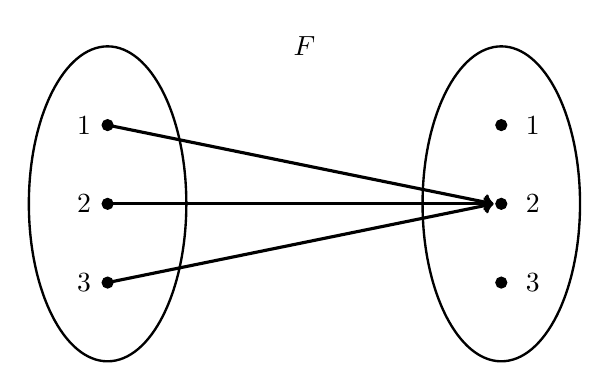
\begin{tikzpicture}
	\node at (2.5,2) {$F$};
	% Ellipses
	\draw[line width=0.03cm] (0,0) circle (1 and 2);
	\draw[line width=0.03cm] (5,0) circle (1 and 2);
	
	% Nodes
	\draw[fill=black] (0,1) circle (0.07);
	\draw[fill=black] (0,0) circle (0.07);
	\draw[fill=black] (0,-1) circle (0.07);
	
	\draw[fill=black] (5,1) circle (0.07);
	\draw[fill=black] (5,0) circle (0.07);
	\draw[fill=black] (5,-1) circle (0.07);
	
	% Arrow
	\draw[line width=0.04cm,->] (0,1) -- (4.9,0);
	\draw[line width=0.04cm,->] (0,0) -- (4.9,0);
	\draw[line width=0.04cm,->] (0,-1) -- (4.9,0);
	
	% Labels
	\node at (-0.3,1) {$1$};
	\node at (-0.3,0) {$2$};
	\node at (-0.3,-1) {$3$};
	
	\node at (5.4,1) {$1$};
	\node at (5.4,0) {$2$};
	\node at (5.4,-1) {$3$};
	\end{tikzpicture}
	\end{minipage}%
	\begin{minipage}[c]{0.40\textwidth}
	\begin{table}[H]
	\centering
	\begin{tabular}{cc}
	$x$ & $G$ \\ \hline
	$1$ & $0$ \\
	$2$ & $2$ \\
	$3$ & $4$ \\
	$4$ & $7$ \\
	$5$ & $0$
	\end{tabular}
	\end{table}
	\end{minipage} \pvspace{1.3cm}

\sol We can see that $F$ is a function because there is only one possible output for each given input: $F(1)= 2$, $F(2)= 2$, and $F(3)= 2$. Similarly, we can see that $G$ is a function because for each possible input, there is only one possible output: $G(1)= 0$, $G(2)= 2$, $G(3)= 4$, $G(4)= 7$, and $G(5)= 0$. 



\newpage



% Problem 3
\problem{10} Determine whether the relations $f(x)= 3x^2 - 4x + 5$ and $g(x, y)= xy^2 - x^2y$ are functions. Be sure to fully justify your answer. Also, find $f(-1)$ and $g(3, -1)$. \pspace

\sol Both $f(x)$ and $g(x, y)$ are functions---for each input $x$ or $(x, y)$, respectively, there is only one possible output, which is obtained by evaluating $f$ at $x$ or $g$ at $(x, y)$ and following order of operations. We have\dots	
	\[
	\begin{aligned}
	f(-1)&= 3(-1)^2 - 4(-1) + 5= 3(1) - (-4) + 5= 3 + 4 + 5= 12 \\[0.3cm]
	g(3, -1)&= 3(-1)^2 - 3^2 (-1)= 3(1) - 9(-1)= 3 + 9= 12
	\end{aligned}
	\]


\end{document}